\documentclass[border=4pt]{standalone}
\usepackage{fontspec}
\usepackage{amsmath}
\usepackage{unicode-math}
\setmainfont{Latin Modern Roman}
\setmathfont{Latin Modern Math}
\usepackage{pgfplots}
\usepackage{pgfplotstable}
\pgfplotsset{compat=1.18}
\usepackage{tkz-euclide}
\usetikzlibrary{arrows.meta,calc,angles,quotes,patterns,3d,backgrounds}
\definecolor{ink}{HTML}{123428}
\definecolor{asy}{HTML}{475569}
\definecolor{mint}{HTML}{86e0bd}
\tikzset{asym/.style={asy, line width=0.9pt, dash pattern=on 5pt off 3.5pt},
         guide/.style={gray!70, line width=0.6pt, densely dotted},
         dot/.style={circle, inner sep=0pt, minimum size=5pt, draw=white, line width=0.5pt},
         odot/.style={circle, inner sep=0pt, minimum size=5.5pt, fill=white, line width=1pt},
         lab/.style={font=\footnotesize, inner sep=1.5pt, text=ink}}
\begin{document}
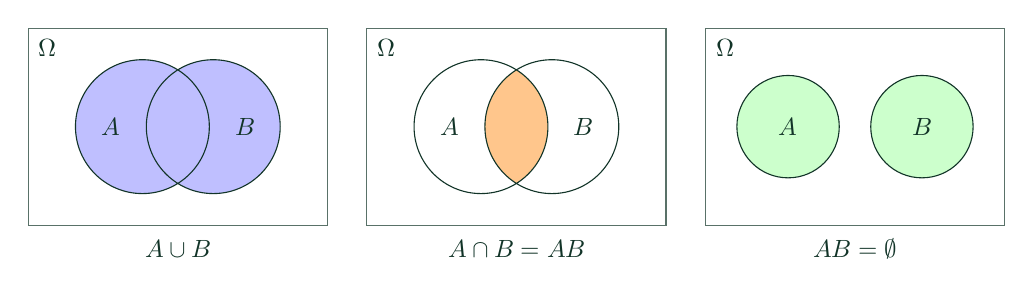
\begin{tikzpicture}[font=\small, every node/.style={text=ink}]
\begin{scope}[shift={(0,0)}]
\draw[ink!70] (-1.9,-1.25) rectangle (1.9,1.25); \node at (-1.65,1.0) {$\Omega$};
\begin{scope} \clip (-0.45,0) circle (0.85); \fill[blue!25] (-2,-2) rectangle (2,2); \end{scope}
\begin{scope} \clip (0.45,0) circle (0.85); \fill[blue!25] (-2,-2) rectangle (2,2); \end{scope}
\draw[ink] (-0.45,0) circle (0.85) (0.45,0) circle (0.85); \node at (-0.85,0) {$A$}; \node at (0.85,0) {$B$}; \node at (0,-1.55) {$A\cup B$};
\end{scope}
\begin{scope}[shift={(4.3,0)}]
\draw[ink!70] (-1.9,-1.25) rectangle (1.9,1.25); \node at (-1.65,1.0) {$\Omega$};
\begin{scope} \clip (-0.45,0) circle (0.85); \fill[orange!45] (0.45,0) circle (0.85); \end{scope}
\draw[ink] (-0.45,0) circle (0.85) (0.45,0) circle (0.85); \node at (-0.85,0) {$A$}; \node at (0.85,0) {$B$}; \node at (0,-1.55) {$A\cap B=AB$};
\end{scope}
\begin{scope}[shift={(8.6,0)}]
\draw[ink!70] (-1.9,-1.25) rectangle (1.9,1.25); \node at (-1.65,1.0) {$\Omega$};
\draw[ink, fill=green!20] (-0.85,0) circle (0.65) (0.85,0) circle (0.65); \node at (-0.85,0) {$A$}; \node at (0.85,0) {$B$}; \node at (0,-1.55) {$AB=\varnothing$};
\end{scope}
\end{tikzpicture}
\end{document}
